\chapter{Marco teórico}
\label{cap:marco}

Aquí van las fichas (Anexo~B), el vocabulario que usa el grupo y la brecha V1--V5. No reescribe el
objeto del §1.4.

\section{Antecedentes de la investigación}
\label{sec:antecedentes}
Catorce trabajos, seis ejes. Las fichas están en el Anexo~B; aquí solo el recorte que usa el
plan. El comentario por paper está en §\ref{sec:estado-arte}.

\begin{enumerate}
  \item \textbf{Madurez de OpenAPI.} En 47 artículos (2011--2020), Casas et al.\ (2021) tratan
        OpenAPI/Swagger como el estándar de facto de las APIs REST: generación, pruebas y
        gobernanza. Coherencia con un modelo de negocio bancario no entra en esa revisión.
  \item \textbf{Correspondencia.} Shvaiko y Euzenat (2005) ordenan el \textit{schema matching}.
        El Bayadh et al.\ (2015), Chandrasekaran y Mago (2022) y Santos Sousa et al.\ (2026)
        cubren alineación ontológica y similitud. Llegan por separado. El score único del par
        contrato--SD se define en este plan, no en esos papers.
  \item \textbf{Dominio e interfaz.} Schmidt y Thiry (2020) revisan 27 estudios de microservicios
        con MDE y DDD. Sirve para no tratar el YAML como si fuera el \ServiceDomain{}.
  \item \textbf{Lo que no es el foco.} Testing, seguridad y selección de servicios (E5 y E6) usan
        OpenAPI para cobertura, vulnerabilidades o ranking por QoS. Eso se excluye en
        \Cref{sec:alcances}.
\end{enumerate}


\section{Bases conceptuales}
\label{sec:bases-conceptuales}
Los términos de abajo se usan siempre con el mismo sentido. La tabla está en
§\ref{sec:glosario}. Cómo se calculan, en §1.4.

\subsection{API REST y contrato OpenAPI}

El archivo que entra al procedimiento es YAML o JSON OpenAPI: \textit{paths}, verbos y
\textit{schemas}. El microservicio que lo implementa no se recibe y no se puntúa. REST ---recurso,
HTTP, JSON--- nombra el estilo de la interfaz. Casas et al.\ (2021) ya fijaron OpenAPI como
estándar de facto; esta sección no vuelve a demostrarlo.

\subsection{Modelo de referencia BIAN}

BIAN divide el banco en \ServiceDomain{}s. Cada dominio publica \Behavior{}s,
\BusinessObject{}s y relaciones de control (Farzi, 2021). En el plan el SD es la referencia contra
la que se compara el contrato. No se evalúa el código del \textit{core} ni el despliegue en un
proveedor.

\subsection{Alineación, coherencia y desalineación}

\textbf{Alineación} es la correspondencia entre el YAML y el SD, medida por \AlignmentScore{}.
Alta o Media se leen como coherencia operativa del par documental. No equivalen a un sello
regulatorio. \textbf{Desalineación} cubre el resto de la \Cref{tab:tipologias}: estructural,
semántica, de modelado o de REST/contrato.

\subsection{Modelo de puntuación}

S, E y C se agregan con pesos $\alpha$, $\beta$ y $\gamma$. La \Cref{fig:bases-conceptuales}
deja el contrato a un lado, el SD al otro y el score en el medio.

\begin{figure}[H]
  \centering
  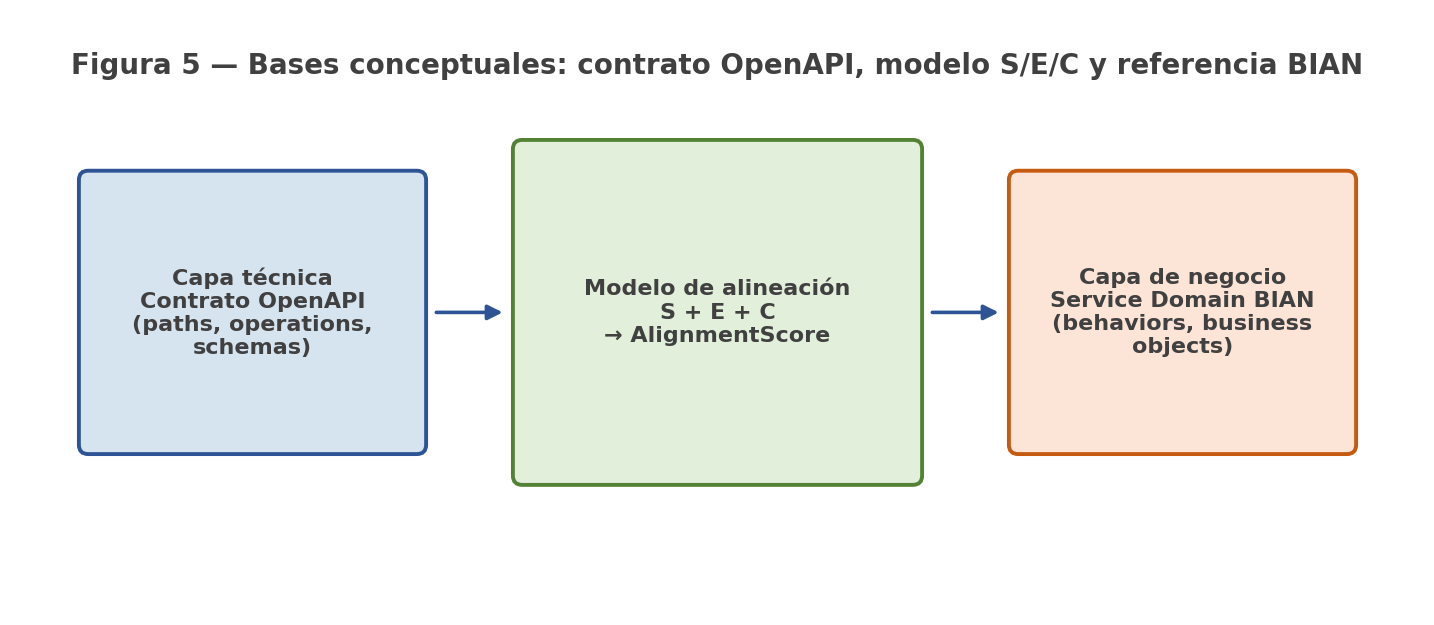
\includegraphics[width=0.92\textwidth]{Figura_05_Bases_Conceptuales}
  \caption{Bases conceptuales: contrato OpenAPI, \ServiceDomain{} BIAN y modelo de alineación S/E/C}
  \label{fig:bases-conceptuales}
\end{figure}


\section{Definición de términos (mapa semántico)}
\label{sec:glosario}
El mapa semántico unifica términos empleados en los capítulos del plan. Cuando un concepto aparece
en varios capítulos, conserva el significado aquí definido.

\begin{table}[H]
  \centering
  \caption{Mapa semántico --- términos clave del plan de tesis}
  \label{tab:glosario}
  \small
  \begin{tabular}{@{}p{0.22\textwidth}p{0.68\textwidth}@{}}
    \toprule
    \textbf{Término} & \textbf{Definición en este plan} \\
    \midrule
    API REST &
    Interfaz que expone recursos y operaciones HTTP con representaciones intercambiables (p.\ ej. JSON). \\
    Contrato OpenAPI &
    Documento YAML/JSON (OpenAPI~3.x) que describe \textit{paths}, \textit{operations} y \textit{schemas} de una API. \\
    BIAN &
    Estándar de arquitectura bancaria que organiza capacidades en \ServiceDomain{}s de referencia. \\
    \ServiceDomain{} &
    Unidad de negocio BIAN descrita por \Behavior{}s, \BusinessObject{}s y relaciones de control. \\
    \Behavior{} &
    Acción o capacidad de negocio definida en un \ServiceDomain{} BIAN. \\
    \BusinessObject{} &
    Entidad de dominio BIAN (p.\ ej. orden de pago, cuenta) referenciada en el modelo. \\
    Objeto de estudio &
    Contrato OpenAPI bancario completo evaluado frente a un \ServiceDomain{} BIAN. \\
    Unidad de análisis &
    Par comparable endpoint/operation/schema $\leftrightarrow$ \Behavior{} / \BusinessObject{}. \\
    Alineación &
    Grado de correspondencia estructural y semántica entre contrato OpenAPI y \ServiceDomain{} BIAN. \\
    Desalineación &
    Divergencia detectable; tipologías: estructural, semántica, modelado, REST/contrato (Tabla~\ref{tab:tipologias}). \\
    Representación normalizada &
    Vista intermedia común (tabular, grafo u ontología) de artefactos OpenAPI y BIAN tras OE1. \\
    \textit{Schema matching} &
    Técnicas de correspondencia entre esquemas o estructuras; base del \StructuralScore{}. \\
    Similitud semántica &
    Medida de equivalencia de significado entre términos/conceptos; base del \SemanticScore{}. \\
    \SemanticScore{} &
    Score $\in [0,1]$ de alineación semántica OpenAPI $\leftrightarrow$ BIAN. \\
    \StructuralScore{} &
    Score $\in [0,1]$ de correspondencia estructural REST $\leftrightarrow$ organización del SD. \\
    \CoverageScore{} &
    Score $\in [0,1]$ de conceptos BIAN cubiertos por el contrato OpenAPI. \\
    \AlignmentScore{} &
    Agregación $\alpha S + \beta E + \gamma C$; clasificación Alta/Media/Baja/Nula. \\
    \textit{Matching} &
    Procedimiento que establece correspondencias entre elementos de dos artefactos normalizados. \\
    \bottomrule
  \end{tabular}
\end{table}


Los términos \SemanticScore{}, \StructuralScore{}, \CoverageScore{} y \AlignmentScore{} se usan
con la convención \textbf{S}, \textbf{E}, \textbf{C} del modelo (véase §1.4 y Anexo~C). El
\StructuralScore{} mide correspondencia REST $\leftrightarrow$ organización del \ServiceDomain{};
no debe confundirse con similitud ontológica genérica ni con métricas de \textit{runtime}.


\section{Bases teóricas}
\label{sec:bases-teoricas}
Estas bases no repiten el estado del arte. Toman de §\ref{sec:estado-arte} los papers que
\textbf{fundan} S, E o C, y los atan a OE1--OE4 y al Capítulo~4.

\subsection{Correspondencia estructural (\textit{schema matching})}

Shvaiko y Euzenat (2005) proponen una taxonomía multidimensional del \textbf{\textit{schema
matching}}: técnicas aproximadas o exactas a nivel de esquema; evidencia sintáctica, semántica o
externa a nivel de elemento y estructura; grado de automatización. El marco es anterior a OpenAPI y
JSON Schema, pero fundamenta el cálculo del \StructuralScore{} al contrastar \textit{paths},
\textit{operations} y \textit{schemas} con la organización de \Behavior{}s y \BusinessObject{}s del
\ServiceDomain{} de referencia.

\subsection{Alineación ontológica y similitud semántica}

El Bayadh et al.\ (2015) clasifican enfoques de \textbf{alineación ontológica} en cuatro familias:
medidas terminológicas, estructurales, extensionales y semánticas. Ninguna medida aislada basta;
combinaciones fijas pueden ser subóptimas, lo que justifica un diseño explícito de pesos en el
modelo S/E/C propuesto.

Chandrasekaran y Mago (2022) trazan la evolución de la \textbf{similitud semántica} desde recursos
léxicos (WordNet) hacia \textit{embeddings} y modelos transformadores. Santos Sousa et al.\ (2026)
catalogan el uso de \textit{embeddings} en ontology matching, señalando limitaciones de supervisión,
escalabilidad y correspondencias complejas.

Estas líneas aportan candidatos para el \SemanticScore{} y, en parte, para estimar cobertura
conceptual (\CoverageScore{}), siempre sobre vocabulario extraído del contrato OpenAPI y del modelo
BIAN normalizado.

\subsection{Representación enriquecida de contratos}

Mainas et al.\ (2023) ---citados en el eje E1--- proponen anotaciones semánticas
(\texttt{x-refersTo}, \texttt{x-kindOf}, etc.), ontología REST/Hydra y traducción OpenAPI
$\rightarrow$ RDF como vía de \textbf{representación enriquecida}.

Evaluaron más de 300 contratos de SwaggerHub con consultas SPARQL. Los tiempos de traducción superan
1~s para YAML de más de 200 líneas. En este plan se consideran como técnicas de normalización
candidatas (Cap.~4), no como definición previa del \SemanticScore{}.

\subsection{Relación con el modelo propuesto}

E2 y E3, solos, no son el producto. El grupo los mete en un procedimiento que entrega S, E, C y
\AlignmentScore{} sobre YAML bancario. Por qué hace falta esa unión: §\ref{sec:brecha}.


\section{Estado del arte por ejes temáticos}
\label{sec:estado-arte}
Seis ejes (E1--E6), los del Anexo~B. No responden la misma pregunta. E1 mira si OpenAPI ya es el
formato con el que se describe REST. E2 y E3 dicen de dónde pueden salir E y S. E4 separa dominio
e interfaz. E5 y E6 quedan al borde: hablan de pruebas y de ranking, no del cruce con un SD. La
\Cref{tab:sintesis-ejes} junta el recorte. El detalle de cada paper está en el Anexo~B.

\subsection{Eje E1 --- OpenAPI como estándar}

Casas et al.\ (2021) mapean 47 artículos primarios entre 2011 y 2020. OpenAPI/Swagger queda como
el estándar de facto para describir REST de forma \textit{machine-readable}. El 68\,\% de esos
trabajos propone herramientas y el 43\,\% mejora la documentación. En ese conjunto no aparece un
modelo de negocio bancario del tipo BIAN.

Mainas et al.\ (2023) anotan contratos (\texttt{x-refersTo}, \texttt{x-kindOf},
\texttt{x-mapsTo}), pasan OpenAPI a RDF y consultan con SPARQL. El corpus supera las 300
especificaciones de SwaggerHub y no es de banca. Lo usamos como pista de representación para S,
no como definición del score.

Santos y Casas (2025), con \textit{Design Science}, catalogan 59 métricas de API Gateway
(latencia, tráfico, errores) en 68 productos. Quedan anotadas para no mezclarlas con la coherencia
documental: miden el \textit{gateway} en producción.

\subsection{Eje E2 --- Matching estructural}

El eje se apoya en un solo paper, Shvaiko y Euzenat (2005). La taxonomía separa \textit{matching}
exacto y aproximado, evidencia sintáctica, semántica o externa, y el grano elemento frente a
estructura. Es anterior a OpenAPI y a JSON Schema. Para el \StructuralScore{} tomamos de ahí el
contraste de \textit{paths} y \textit{schemas} contra \Behavior{}s y \BusinessObject{}s. La
taxonomía no trae una métrica lista para el par bancario; el cálculo se escribe en el
Capítulo~\ref{cap:metodologia}.

\subsection{Eje E3 --- Matching semántico y ontologías}

El Bayadh et al.\ (2015), Chandrasekaran y Mago (2022) y Santos Sousa et al.\ (2026) no trabajan
contratos bancarios. El primero advierte que una sola medida de alineación ontológica se queda
corta; las cuatro familias están en §\ref{sec:bases-teoricas} y no se repiten aquí. Chandrasekaran
y Mago recorren la similitud desde WordNet hasta \textit{transformers}. Santos Sousa et al.\ (2026)
listan, para \textit{embeddings} en \textit{ontology matching}, tres límites que nos importan:
supervisión, escala y correspondencias complejas. Esos tres papers son candidatos de técnica para
S y, en parte, para C.

\subsection{Eje E4 --- Microservicios e interfaces}

Schmidt y Thiry (2020) parten de 715 registros y se quedan con 27 estudios primarios (2013--2019)
sobre cómo se identifican microservicios con MDE y DDD. El dato que usamos es la separación: el
\ServiceDomain{} puede ser la referencia de negocio y la API, la capa que lo expone. En su muestra
casi no hay trabajos que integren MDE y DDD a la vez. No reportan una métrica de coherencia
contrato--BIAN. El eje solo justifica que las dos capas no se confundan.

\subsection{Eje E5 --- Testing y calidad API (borde)}

Cinco papers, y OpenAPI entra como insumo de prueba. Ehsan et al.\ (2022) cubren 16 artículos de
testing RESTful; la métrica que más se repite es \textit{code coverage}. Golmohammadi et al.\
(2024) leen 92 papers (\textit{fuzzing}, \textit{search-based}, \textit{model-based}) que generan
casos sobre endpoints ya desplegados. Otieno y Araka (2026) ponen aprendizaje automático en el
testing y señalan \textit{datasets} chicos. Tanveer et al.\ (2025) van a vulnerabilidades.
Vitorino et al.\ (2025), a datos adversariales.

Ese cuerpo es el que deja fuera del plan el testing, la seguridad y la QoS operativa
(\Cref{sec:alcances}).

\subsection{Eje E6 --- Selección y recomendación de servicios}

Mahanra Rao et al.\ (2025) revisan 25 estudios (2020--2024, PRISMA) que usan BERT o
\textit{transformers} para elegir servicios web según QoS. La representación semántica de las
descripciones se parece a lo que haríamos en S, pero el resultado es un ranking, no un contraste
contra un \ServiceDomain{}. Reportan costo de cómputo alto, \textit{datasets} cortos y poca
interpretabilidad. Queda como vecino, no como técnica del modelo.

\begin{table}[H]
  \centering
  \caption{Síntesis del estado del arte por ejes (E1--E6)}
  \label{tab:sintesis-ejes}
  \small
  \begin{tabular}{@{}p{0.06\textwidth}p{0.20\textwidth}p{0.22\textwidth}p{0.16\textwidth}p{0.24\textwidth}@{}}
    \toprule
    \textbf{Eje} & \textbf{Papers} & \textbf{Hallazgo principal} & \textbf{Aporte S/E/C} & \textbf{Vacío OpenAPI--BIAN} \\
    \midrule
    \textbf{E1} &
    Casas 2021; Mainas 2023; Santos y Casas 2025 &
    OpenAPI consolidado; enriquecimiento semántico posible &
    S (Mainas); contexto estándar &
    Sin vínculo con \ServiceDomain{} BIAN \\
    \textbf{E2} &
    Shvaiko 2005 &
    Taxonomía de \textit{schema matching} &
    E &
    Sin aplicación REST/banca/BIAN \\
    \textbf{E3} &
    El Bayadh 2015; Chandrasekaran 2022; Santos Sousa 2026 &
    Ontología matching + embeddings + STS &
    S; C parcial &
    Sin contratos OpenAPI ni dominio bancario \\
    \textbf{E4} &
    Schmidt 2020 &
    Dominio (DDD/MDE) $\rightarrow$ microservicios &
    Contexto dominio$\rightarrow$interfaz (no \StructuralScore{} operativo) &
    Sin métrica de alineación \\
    \textbf{E5} &
    Ehsan 2022; Golmohammadi 2024; Otieno 2026; Tanveer 2025; Vitorino 2025 &
    Testing, ML-test, seguridad &
    Delimitación (fuera de foco) &
    Orthogonal al \AlignmentScore{} \\
    \textbf{E6} &
    Mahanra Rao 2025 &
    BERT + QoS en selección de servicios &
    S parcial &
    Recomendación $\neq$ alineación BIAN \\
    \bottomrule
  \end{tabular}
\end{table}


El Anexo~B baja objetivo, técnicas, métricas y límites de cada paper. Esta sección no lo duplica.


\section{Brecha y oportunidad de investigación}
\label{sec:brecha}
\subsection{Qué sí cubre la literatura revisada}

Los catorce papers, leídos en cruz y no eje por eje, dejan esto:

\begin{enumerate}
  \item OpenAPI es el formato con el que se especifica REST (E1). Casas et al.\ (2021) lo muestran
        en 47 artículos; Mainas et al.\ (2023) prueban que se puede enriquecer semánticamente sobre
        corpus reales.
  \item Hay marcos para cruzar esquemas (E2) y para medir significado (E3). Shvaiko y Euzenat
        (2005) y El Bayadh et al.\ (2015) se pueden reutilizar; Santos Sousa et al.\ (2026) ya
        documentaron dónde fallan los \textit{embeddings}.
  \item E4 separa dominio e interfaz. Schmidt y Thiry (2020) hablan de microservicios; BIAN juega
        el mismo papel como referencia de capacidad.
  \item E5 es otro oficio. Ehsan et al.\ (2022) y Golmohammadi et al.\ (2024) usan OpenAPI para
        probar APIs vivas. Eso recorta el plan: calidad operativa $\neq$ coherencia con BIAN.
  \item E6 (Mahanra Rao et al., 2025) rankea servicios por QoS. Consume descripciones; no pregunta
        si el YAML bancario refleja un \ServiceDomain{}.
\end{enumerate}

La pregunta del grupo sigue sin respuesta en ese corpus: \textit{¿en qué medida un contrato
OpenAPI bancario refleja un \ServiceDomain{} BIAN, y cómo se puntúa eso de modo que otro pueda
repetirlo?}

\subsection{Vacíos identificados}

\begin{table}[H]
  \centering
  \caption{Vacíos identificados en la literatura (V1--V5)}
  \label{tab:vacios}
  \small
  \begin{tabular}{@{}p{0.14\textwidth}p{0.38\textwidth}p{0.38\textwidth}@{}}
    \toprule
    \textbf{Vacío} & \textbf{Evidencia en el review} & \textbf{Implicación para la tesis} \\
    \midrule
    \textbf{V1 --- Intersección OpenAPI $\cap$ BIAN} &
    Ningún paper del corpus junta ambos artefactos en banca &
    Objeto: contrato OpenAPI vs.\ SD BIAN \\
    \textbf{V2 --- Métrica integrada} &
    E2 y E3 dan técnicas sueltas; E1 no mide alineación &
    Producto: S, E, C y \AlignmentScore{} \\
    \textbf{V3 --- Cobertura de conceptos} &
    La cobertura ontológica no se calcula sobre \BusinessObject{} BIAN en OpenAPI &
    \CoverageScore{} \\
    \textbf{V4 --- Procedimiento reproducible} &
    Mainas et al.\ (2023): RDF, sin score ni nivel &
    Diseño del Cap.~4 \\
    \textbf{V5 --- Gobernanza documental} &
    E5 y E6: \textit{runtime} o ranking, no deriva contrato--modelo &
    Medir antes del despliegue \\
    \bottomrule
  \end{tabular}
\end{table}


La \Cref{fig:brecha} pasa de E1--E6 a los vacíos V1--V5.

\begin{figure}[H]
  \centering
  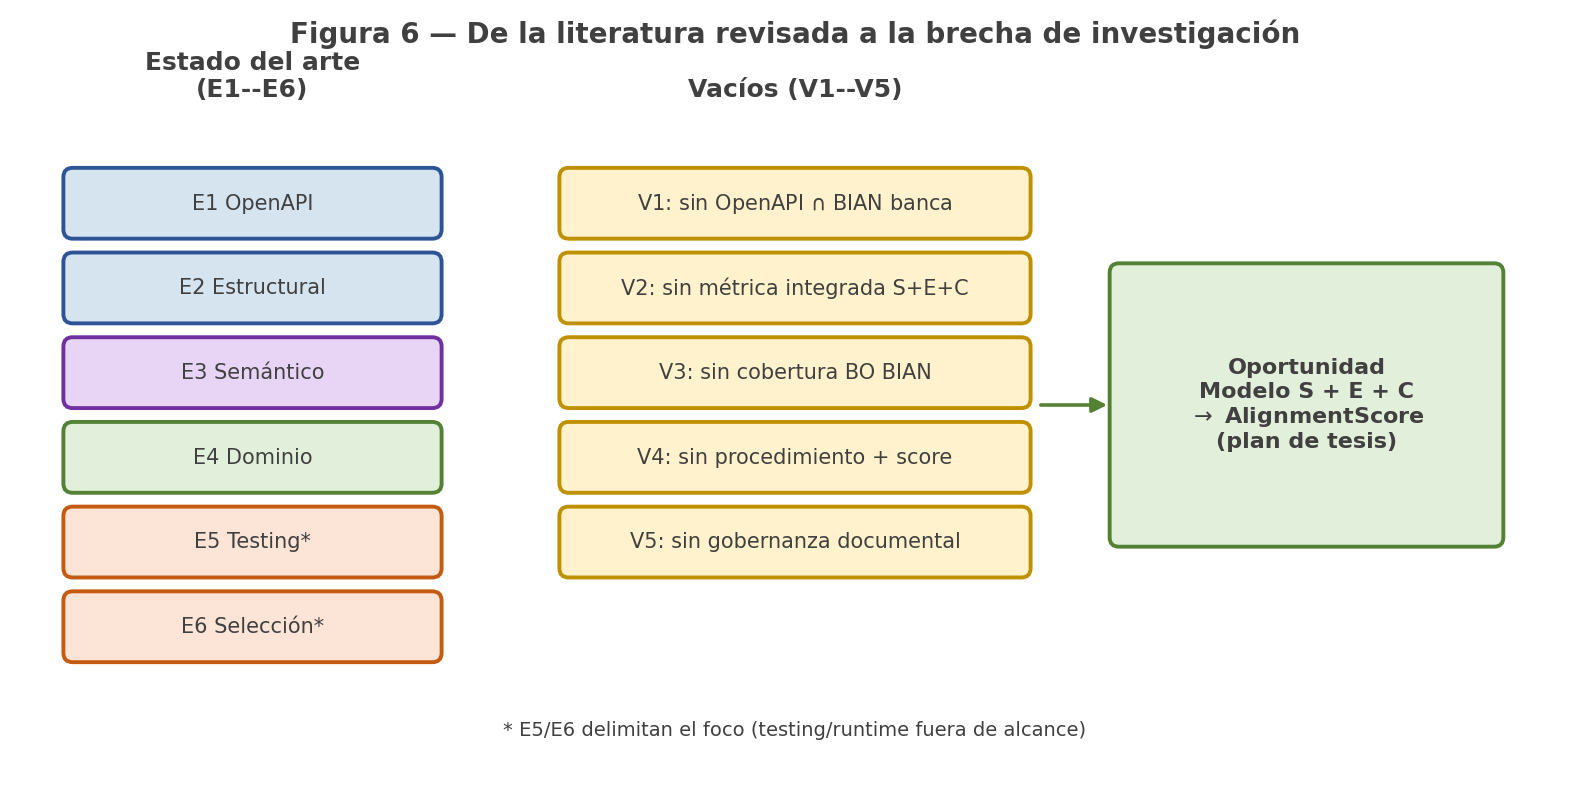
\includegraphics[width=0.95\textwidth]{Figura_06_Brecha}
  \caption{De la literatura revisada (E1--E6) a la brecha de investigación (V1--V5)}
  \label{fig:brecha}
\end{figure}

\subsection{Oportunidad de investigación}

Cinco fases. Primera: escribir el modelo. Luego OE1 (normalizar), OE2--OE3 (E y S; C junto a
OE4) y el \AlignmentScore{} con umbrales Alta / Media / Baja / Nula.

Guía~1 se queda en el papel (\Cref{sec:alcances}). Cubre V1--V4 sobre documentos. No cubre
testing (E5) ni un sello de cumplimiento.


V1--V5 quedan así recortados. Las técnicas pasan al Capítulo~\ref{cap:metodologia}. El problema
tecnológico de la matriz (Anexo~C) no se confunde con este capítulo.
